\documentclass[11pt]{amsart}
\usepackage{geometry}                % See geometry.pdf to learn the layout options. There are lots.
\geometry{letterpaper}                   % ... or a4paper or a5paper or ... 
%\geometry{landscape}                % Activate for for rotated page geometry
%\usepackage[parfill]{parskip}    % Activate to begin paragraphs with an empty line rather than an indent
\usepackage{graphicx}
\usepackage{amssymb}
\usepackage{epstopdf}
\DeclareGraphicsRule{.tif}{png}{.png}{`convert #1 `dirname #1`/`basename #1 .tif`.png}

\usepackage{amsmath}
\usepackage{algorithm}
\usepackage[noend]{algpseudocode}

\makeatletter
\def\BState{\State\hskip-\ALG@thistlm}
\makeatother

\title{KD-tree Implemention and performance}
%\author{The Author}
%\date{}                                           % Activate to display a given date or no date

\begin{document}
\maketitle
%\section{}
%\subsection{}

The various components used in this project are as follows:

\begin{list}{\labelitemi}{\leftmargin= 1.4cm} \setlength\itemsep{1em}

\item \textbf{Sample matrix}: Input samples are represented as a matrix $M \in R^{m \times n}$, where we have $m$ samples and $n$ dimensions and $M_{ij}$ represents the value for $i^{th}$ sample in $j^{th}$ dimension. We use Eigen library \cite{Guennebaud:2010aa} to represent this matrix.

\item \textbf{Segment}: Segment is the logical partitioning of samples that is used by the KD-tree algorithm during tree construction. Example of segments is shown in Figure \ref{fig:segment}. The six samples are stored in memory as a Eigen matrix and shared by all segments. Each segment contains a vector of sample ids that are present in the segment. The first segment contains all the sample ids. 

After a split, during tree building process, we get two almost equal segments which contains a reference to the main matrix and have a vector of sample ids that indicate the samples from matrix with belong in the segment. Partitioning samples this way allows us to develop recursive or parallel algorithms to build trees efficiently. 

\item \textbf{Split}: This contains the information that we need to split samples into segments. This is created during tree building process and used when we are searching for a query in the tree. Every internal node in the tree contains this split object. Split contains the following details (Figure \ref{fig:bounding_box}):
\vspace{1.5 mm}
\begin{enumerate} \setlength\itemsep{0.5em}
\item Split dimension ($d_{t+1}$): This the dimension along which we will be splitting the samples at ${(t+1)}^{th}$ node during search.
\item Split point: This is the point that is used to split the samples in the segment into almost equal size. If the number of points in the segment are odd then the split point is the one in middle otherwise it is the average of the 2 points in the middle. This is the point in the centre of Figure  \ref{fig:bounding_box}.
\item Bounds:  These define the boundaries of left and right segments generated after the current segment is split. We store: (i) min point, which is the min value in all dimensions for samples in the segment; and, (ii) max point, which is the max value in all dimensions for samples in the segment.
\end{enumerate}
\item \textbf{Split Dimension Selector}: This is used to select the dimension that will be used to split the samples next. The selector supports 2 methods:
\vspace{1.5 mm}
\begin{enumerate}\setlength\itemsep{0.5em}
\item Cycle through axis: This method cycles through dimensions. 
\[ d_{t+1} = (d_{t} + 1)  \% n \]
\item Highest range axis: This method selects a dimension that has the maximum spread of points.
\[ d_{t+1} = \operatorname{arg\,max}_j  (\text{max\_value\_along j - min\_value\_along j})\] 
\end{enumerate}

\item \textbf{Split Point Selector}: This is used to select the threshold that will be used to separate points. These methods return the same value but the complexity of finding them is different depending on the method. This selector supports 2 methods:
\vspace{1.5 mm}
\begin{enumerate}\setlength\itemsep{0.5em}
\item Median: Sorts the values for dimensions we are splitting across and picks the median. This has a complexity of $O(nlogn)$. 
\item Median \-of \-median: This uses a selection algorithm that picks the $k^{th}$ biggest item with $O(n)$ complexity.
\end{enumerate}

\item \textbf{KD-tree}: The KD-tree object is represented as an array of nodes. A node can either be an  internal node containing information of how to split samples or a leaf node that contains id for a sample. The array is indexed from 0, so for internal nodes at index $k$, the left child is at $2k + 1$ and the right child is at $2k + 2$.

\end{list}

\begin{figure}[t!]
\centering
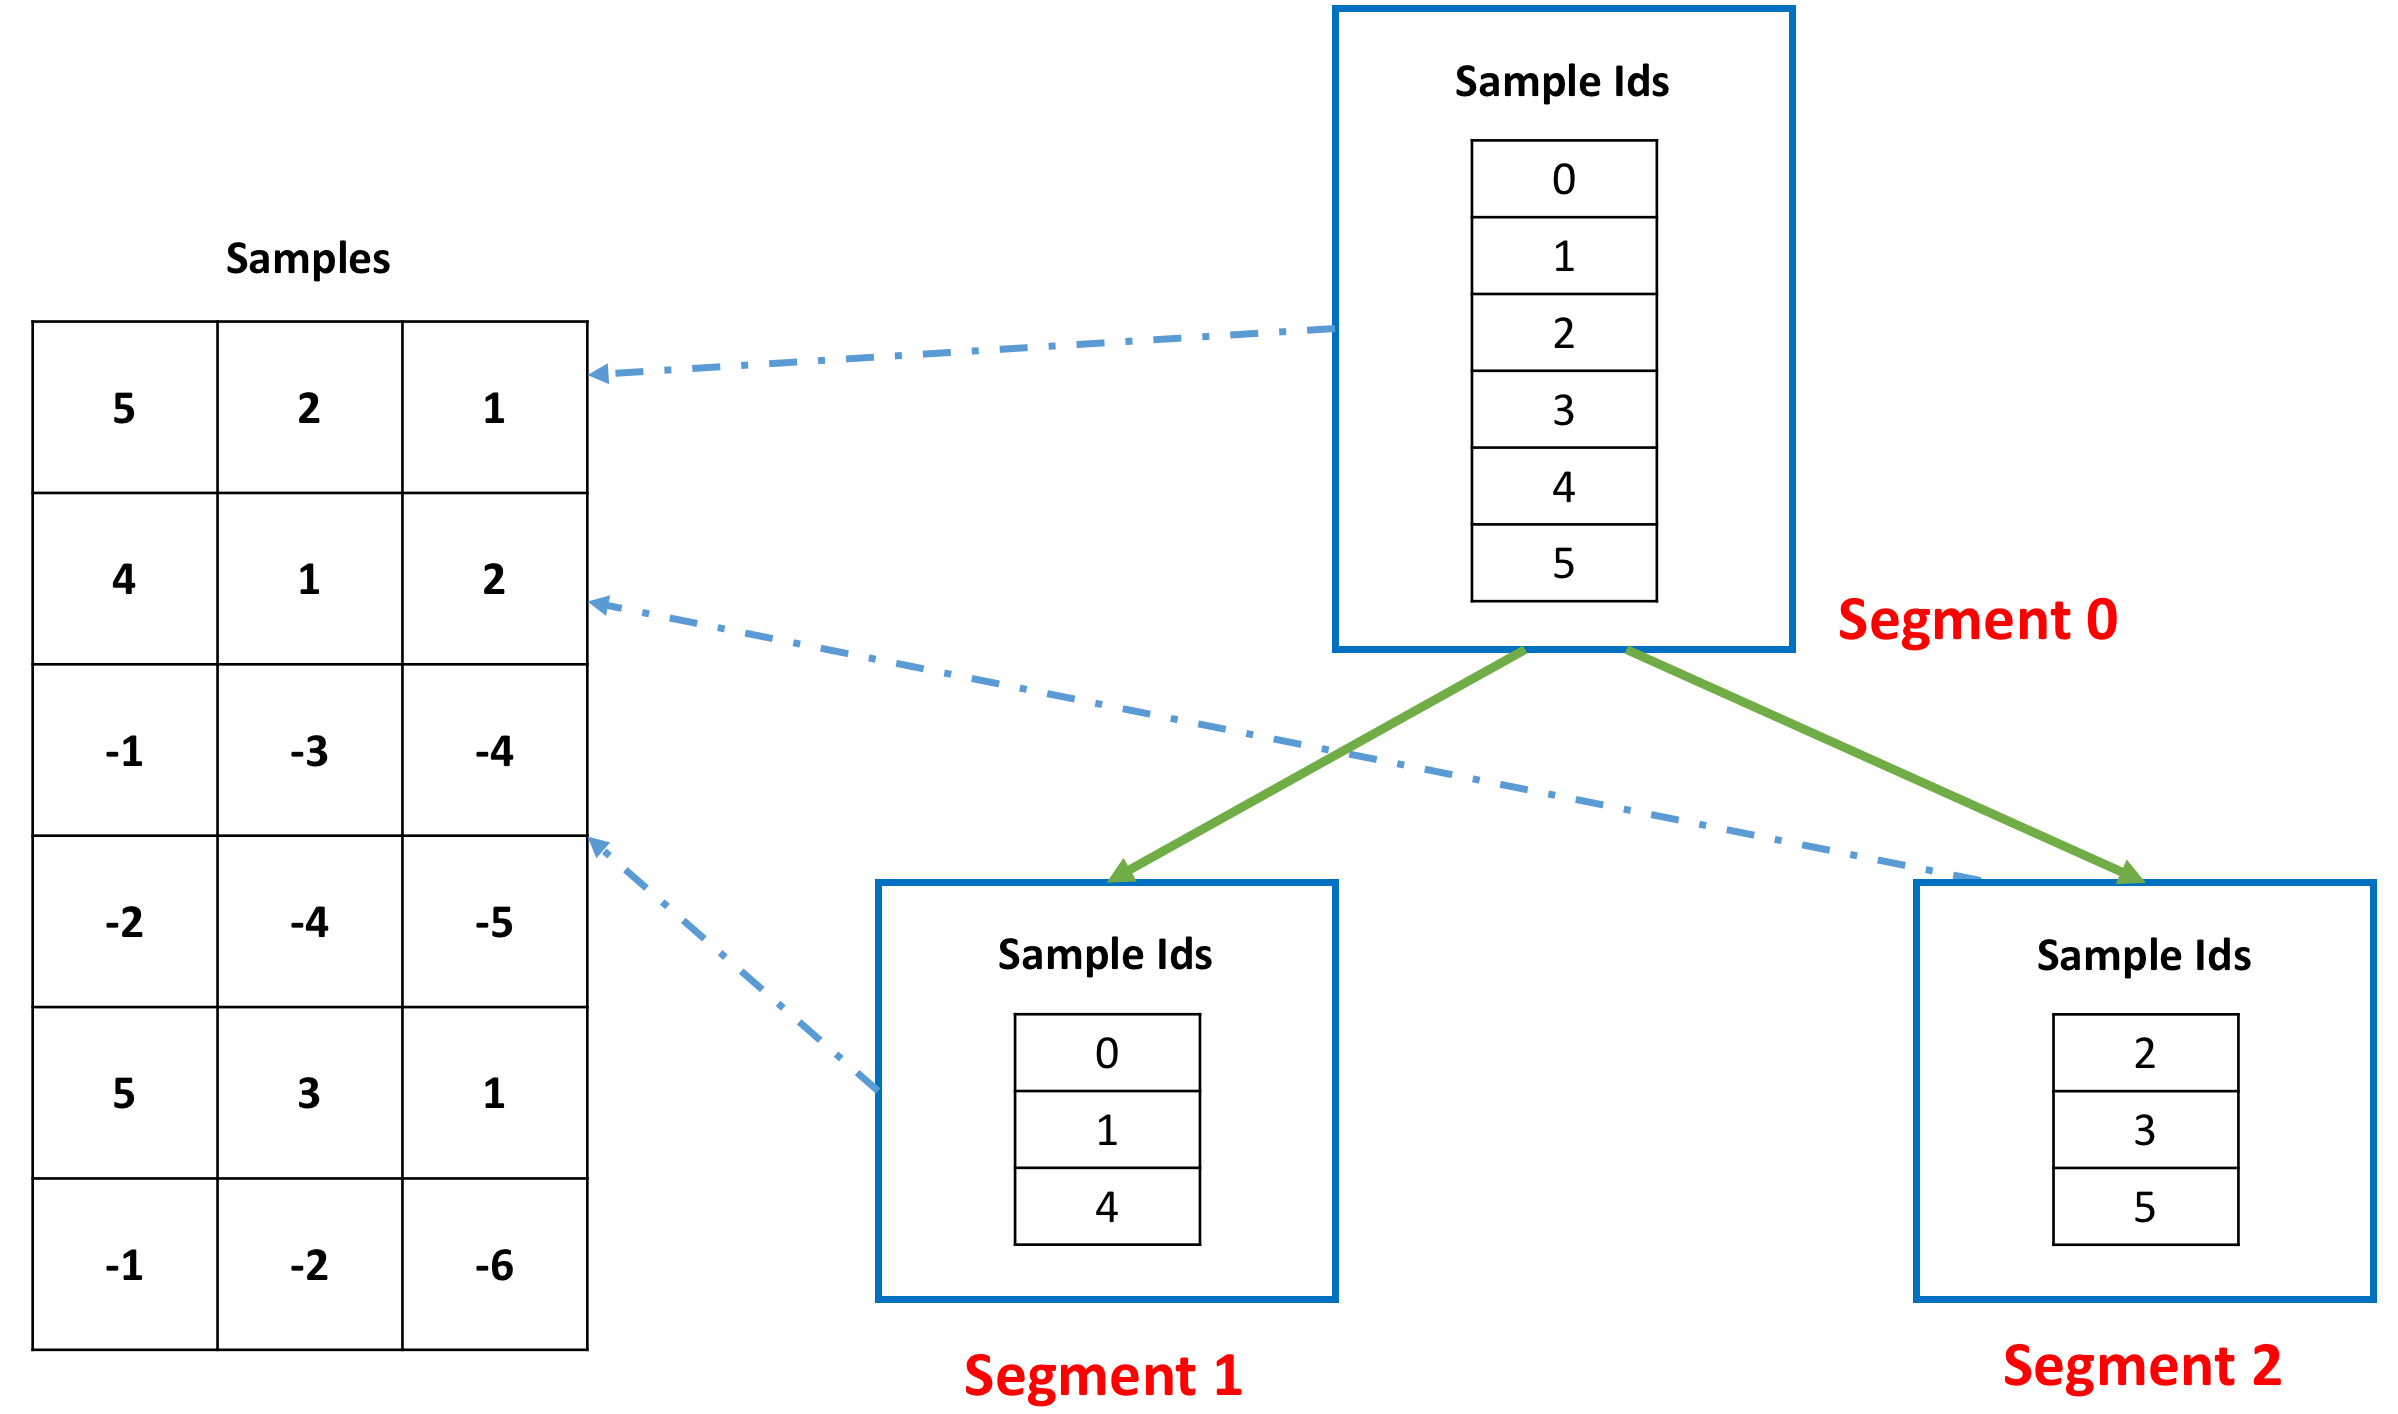
\includegraphics[width=\linewidth]{images/segment}
\caption{Example of how samples are stored in an Eigen matrix and then shared between segments.}
\label{fig:segment}
\end{figure}

\begin{figure}[t!]
\centering
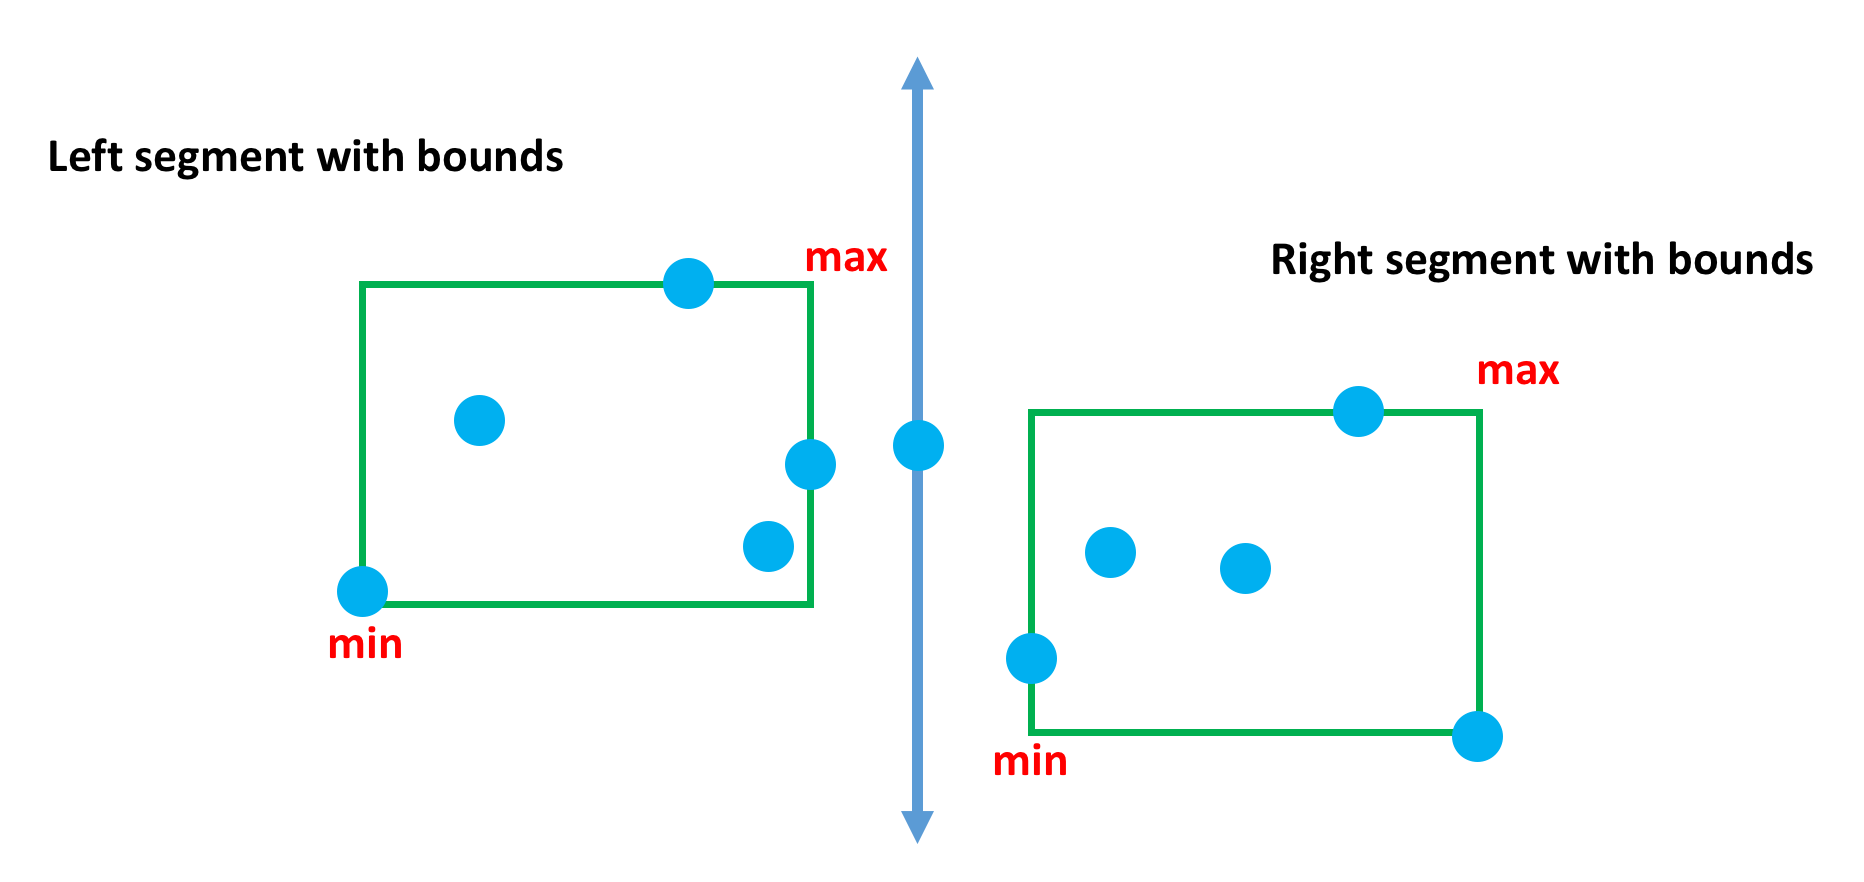
\includegraphics[width=\linewidth]{images/bounding_box}
\caption{Example of a split, with split point, left and right bounding boxes.}
\label{fig:bounding_box}
\end{figure}

\begin{algorithm}
\caption{Tree building algorithm (recursive)}
\label{tree_building_recursive}
\begin{algorithmic}[1]
\State Load samples
\State Initialize KD-tree as an array of nodes of size $2^{\left \lfloor{log_{2}(\text{num samples})}\right \rfloor + 1 }$ 
\State Create Segment $S_0$ which contains all samples
\State 
\State BuildTreeRecursive($S_0$)
\State 
\Procedure{BuildTreeRecursive}{Segment S}
\If {S contains just one sample} 
\State Create a leaf node with one sample and insert it to the KD-tree
\Else
\State Get dimension to split by using dimension selector.
\State Get the split threshold using split point selector.
\State Insert an internal node with split information into KD-tree.
\State
\State Generate the segments:
\State $S_l \gets $ all samples less than split threshold; and
\State $S_r \gets $  all samples greater than the split threshold
\State
\State BuildTreeRecursive($S_l$)
\State BuildTreeRecursive($S_r$)
\EndIf
\EndProcedure
\end{algorithmic}
\end{algorithm}

\begin{algorithm}
\caption{Tree building algorithm (parallel)}
\label{tree_building_parallel}
\begin{algorithmic}[1]
\State Load samples
\State Initialize KD-tree as an array of nodes of size $2^{\left \lfloor{log_{2}(\text{num samples})}\right \rfloor + 1 }$ 
\State Create Segment $S_0$ which contains all samples
\State 
\State BuildTreeParallel($S_0$)
\State
\Procedure{BuildTreeParallel}{Segment S}
\State Create a thread pool $P$
\State Initialize a thread-safe queue Q
\State Push segment onto queue: $Q \gets Q + S$
\While {Q is not empty}
\State $p \gets \text{next free thread in P}$
\State $S_c \gets \text{Last item from } Q$ \hspace{0.5in}// mimics stack
\State $p \rightarrow$  ProcessSegment($S_c$, $Q$)
\EndWhile
\EndProcedure
\State
\Procedure{ProcessSegment}{Segment S, Queue Q}
\If {S contains just one sample} 
\State Create a leaf node with one sample and insert it to the KD-tree
\Else
\State Get dimension to split by using dimension selector.
\State Get the split threshold using split point selector.
\State Insert an internal node with split information into KD-tree.
\State
\State Generate the segments:
\State $S_l \gets $ all samples less than split threshold; and
\State $S_r \gets $  all samples greater than the split threshold
\State
\State $Q \gets Q + S_r$
\State $Q \gets Q + S_l$
\EndIf
\EndProcedure
\State 
\end{algorithmic}
\end{algorithm}

\begin{algorithm}
\caption{Query searching algorithm}
\label{query_searching}
\begin{algorithmic}[1]
\State Load samples
\State Load KD-tree as an array of nodes
\State
\Procedure{SearchQuery}{Query q}
\State $N \gets \text{First node in KD-tree}$
\State Push node onto queue: $Q \gets Q + N$
\State
\State Initialize current nearest neighbor $N^\prime$ and Euclidean distance from that neighbor $d^\prime$
\State $N^\prime \gets N$
\State $d^\prime \gets \infty$
\State
\While {Q is not empty}
\State $N_i \gets \text{Last item from } Q$ \hspace{0.5in}// mimics stack
\If {$N_i$ is a leaf node} 
\State $d \gets distance(N_i, q)$
\If {$d \leq d^\prime$}
\State $d^\prime \gets d$
\State $N^\prime \gets N_i$
\EndIf
\Else
\State Get current split: $P \gets N.split$
\State $d_{left} \gets distance(P.leftBounds,\text{ } q)$ 
\State $d_{right} \gets distance(P.rightBounds,\text{ } q)$ 
\State
\State $leftIsCloser \gets d_{left} \leq d^\prime$ 
\State $rightIsCloser \gets d_{right}  \leq d^\prime$ 
\State
\If {$leftIsCloser$ \&\& $rightIsCloser$} 
\State Order in which to explore next side is decided by which is the closer side.
\If { $d_{left} \leq d_{right}$}
\State $Q \gets Q + P.rightNode$
\State $Q \gets Q + P.leftNode$
\Else
\State $Q \gets Q + P.leftNode$
\State $Q \gets Q + P.rightNode$
\EndIf
\ElsIf {$leftIsCloser$} 
\State $Q \gets Q + P.leftNode$
\ElsIf {$rightIsCloser$} 
\State $Q \gets Q + P.rightNode$
\EndIf
\EndIf
\EndWhile
\EndProcedure
\end{algorithmic}
\end{algorithm}

 \bibliography{sigproc}
 \bibliographystyle{unsrt}

\end{document}  